\section{Schaltvorgänge}
\subsection{Berechnen von Schaltvorgänge im Bildbereich}
\subsubsection{Laplacetransformation der Differentialgleichung}
Aufgrund der Eigenschaften der Laplacetransformation wird aus einer
DGL im Zeitbereich eine algebraische Gleichung im Bildbereich.

\textbf{Differentiation im Zeitbereich}:
\[
	\frac{d}{dt}x(t) \ \laplace\ s\cdot\underline{X}(s)-x(0^+)
\]
\[
	\frac{d^2}{dt^2}x(t) \ \laplace\ s^2\cdot\underline{X}(s)-s\cdot x(0^+)-\frac{dx}{dt}(0^+)
\]


\subsubsection{Schaltvorgänge mit ungeladenen Energiespeichern}
\begin{enumerate}
	\item Das Eingangssignal wird mit der Laplacetransformation in den
	      Bildbereich transformiert.
    \item Die Übertragungsfunktion wird aus dem Schaltbild nach dem
        Schaltvorgang mit komplexer Wechselstromrechnung bestimmt
    \item Das Ausgangssignal wird im Bildbereich berechnet: $\underline{Y}(s) =
        \underline{X}(s)\cdot \underline{H}(s)$
    \item Rücktransformation in den Zeitbereich mit Hilfe der Tabellen
    \item \textbf{NUR:} wenn alle Energiespeicher zum zeitpunkt $t=0$
        energielos sind:
        \subitem[i] Kondensatoren ungeladen
        \subitem[ii] Spulen stromlos
\end{enumerate}
\subsubsection{Schaltvorgänge mit geladenen Energiespeichern}
\begin{enumerate}
    \item Erstellen eines Ersatzschaltbild für den Schaltkreis nach dem
        Schaltvorgang:
        \begin{itemize}
            \item Induktivitäten mit Anfangsstrom
                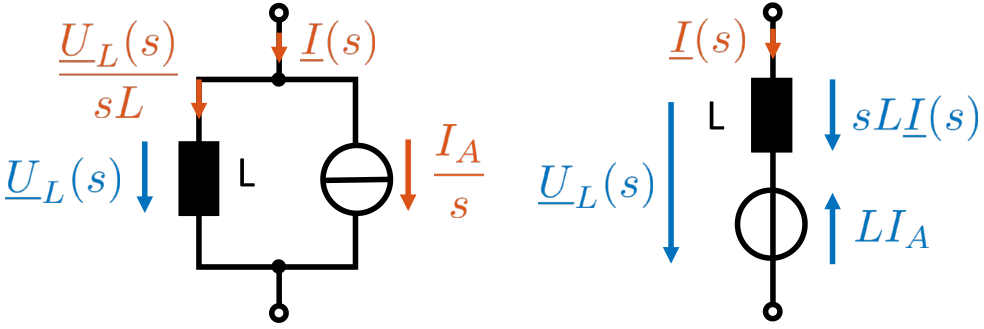
\includegraphics[width=0.40\textwidth]{Bilder/ESB_Fuer_stromfuehrende_Induktivitaet}
                \begin{align*}
                    \underline{U}_L(s) &= L\cdot(s\cdot\underline{I}_L(s)-\underbrace{i_L(t=0)}_{I_A})\\
                    \underline{I}_L(s) &= \frac{\underline{U}_L(s)}{sL}+\frac{I_A}{s}
                \end{align*}
            \item Kapazitäten mit Anfangsspannung (Vorladung):
                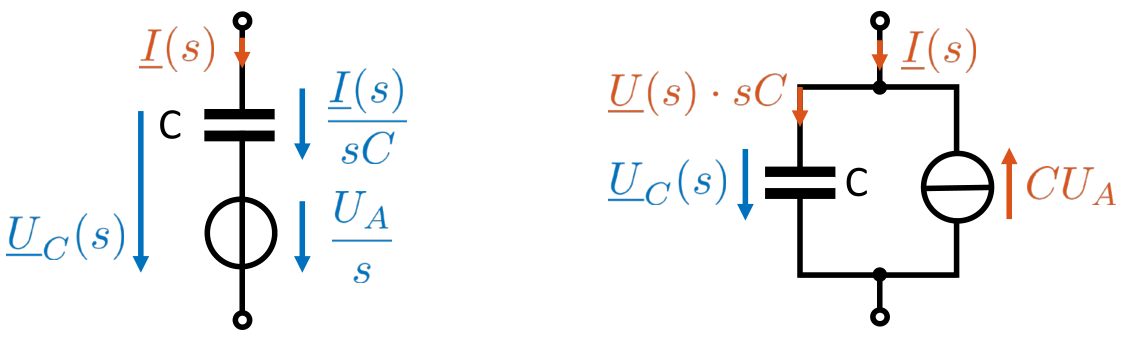
\includegraphics[width=0.40\textwidth]{Bilder/ESB_Fuer_geladene_Kapazitaet}
                \begin{align*}
                    \underline{I}_C(s) &= C\cdot(s\cdot\underline{U}_C(s)-\underbrace{u_C(t=0)}_{U_A})\\
                    \underline{U}_C(s) &= \frac{\underline{I}_C(s)}{sC}+\frac{U_A}{s}
                \end{align*}
        \end{itemize}
    \item Die Übertragungsfunktion wird aus dem Ersatzschaltbild mit komplexer
        Wechselstromrechnung bestimmt
    \item Das Eingangssignal wird mit der Laplacetransformation in den Bildbereich
        transformiert.
    \item Das Ausgangssignal wird im Bildbereich berechnet: $\underline{Y}(s) =
        \underline{X}(s)\cdot \underline{H}(s)$
    \item Rücktransformation in den Zeitbereich mit Hilfe der Tabellen
\end{enumerate}
